\section{Results}
\label{sec:Results}

%%%%%%%%%%%%%%%%%%%%%%%%%%%%%%%%%%%%%%%%%%%%%%%%%%%%%%%%%%%%%%%%%%%%%%%%%%%%%%%%%%%%
\subsection{Ground Testing}
\textcolor{red}{CL  - Discuss results from ground testing.}
During each run of the ground test, a Pixhawk data acquisition system was used to collect data on the motion of the drogue while in flight. This data was then converted to Euler angles and axial accelerations for additional analysis. Fig. \ref{fig:Run2Euler} shows the Euler angles from the drogue in Configuration 1, while Fig. \ref{fig:Run4Euler} shows the drogue in Configuration 2 and Fig. \ref{fig:Run6Euler} shows the drogue in Configuration 3. Though this figure shows all three Euler angles, analysis was focused on the Roll angle, which is the top plot in all three figures.

\begin{figure}
	\centering
	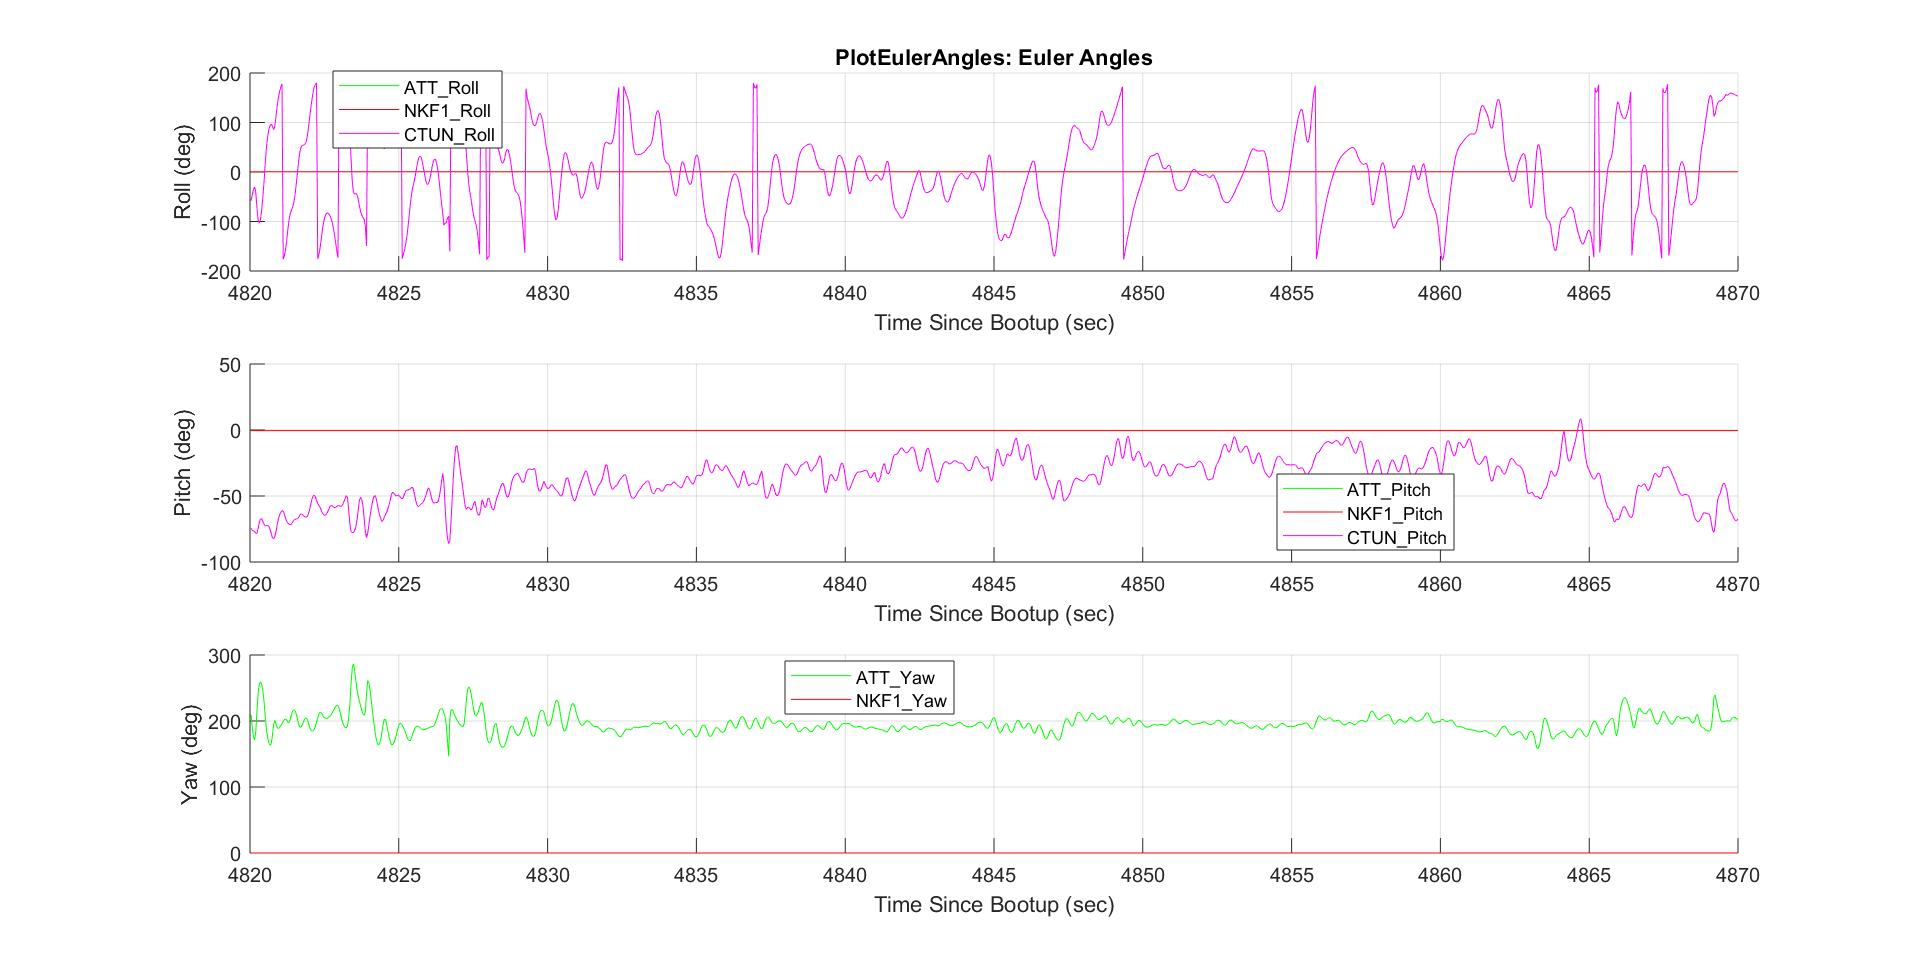
\includegraphics[width=1\linewidth]{./images/Run2_Euler}
	\caption{Euler angles in Configuration 1.} %way to classify fins
	\label{fig:Run2Euler}
\end{figure}

Each test includes a very short window of time when the drogue was moving through the air at a high enough speed to simulate actual flight tests. For Fig. \ref{fig:Run2Euler}, was identified as occurring approximately between times 4830 $sec$ and 4865 $sec$. Because the truck reached lower speeds during this test than the other tests, the flight time for this run was significantly shorter than the other tests. When looking at the Euler angles in this time frame, complete rolls by the drogue are shown by vertical lines stretching from 200 $deg$ to -200 $deg$. During this time frame 4 rolls were identified. 

%%%%%%%%%%%%%%%%%%%%%%%%%%%%%%%%%%%%%%%%%%%%%%%%%%%%%%%%%%%%%%%%%%%%%%%%%%%%%%%%%%%%

%%%%%%%%%%%%%%%%%%%%%%%%%%%%%%%%%%%%%%%%%%%%%%%%%%%%%%%%%%%%%%%%%%%%%%%%%%%%%%%%%%%%
\subsection{Flight Testing}
\textcolor{red}{CL  - Discuss results from flight testing.}

%%%%%%%%%%%%%%%%%%%%%%%%%%%%%%%%%%%%%%%%%%%%%%%%%%%%%%%%%%%%%%%%%%%%%%%%%%%%%%%%%%%%
